% Lecture Template for ME3001-001-Tristan Hill - Spring 2017 - Fall 2017
% 
% Mechanical Engineering Analysis with MATLAB
%
% Numerical Solutions to Oridnary Differential Equations - Lecture 1


% Document settings
\documentclass[11pt]{article}
\usepackage[margin=1in]{geometry}
\usepackage[pdftex]{graphicx}
\usepackage{multirow}
\usepackage{setspace}
\usepackage{hyperref}
\usepackage{color,soul}
\usepackage{fancyvrb}
\usepackage{framed}
\usepackage{wasysym}
\usepackage{multicol}

\pagestyle{plain}
\setlength\parindent{0pt}
\hypersetup{
    bookmarks=true,         % show bookmarks bar?
    unicode=false,          % non-Latin characters in Acrobat’s bookmarks
    pdftoolbar=true,        % show Acrobat’s toolbar?
    pdfmenubar=true,        % show Acrobat’s menu?
    pdffitwindow=false,     % window fit to page when opened
    pdfstartview={FitH},    % fits the width of the page to the window
    pdftitle={My title},    % title
    pdfauthor={Author},     % author
    pdfsubject={Subject},   % subject of the document
    pdfcreator={Creator},   % creator of the document
    pdfproducer={Producer}, % producer of the document
    pdfkeywords={keyword1} {key2} {key3}, % list of keywords
    pdfnewwindow=true,      % links in new window
    colorlinks=true,       % false: boxed links; true: colored links
    linkcolor=red,          % color of internal links (change box color with linkbordercolor)
    citecolor=green,        % color of links to bibliography
    filecolor=magenta,      % color of file links
    urlcolor=blue           % color of external links
}

% assignment number 
\newcommand{\NUM}{1} 
\newcommand{\VSpaceSize}{2mm} 
\newcommand{\HSpaceSize}{2mm} 
\newcommand{\VSPC}{15mm} 


\definecolor{mygray}{rgb}{.6, .6, .6}
% [153,50,204] - dark orchid
\definecolor{mypurple}{rgb}{0.6,0.1961,0.8}
%[139,69,19] - saddle brown
\definecolor{mybrown}{rgb}{0.5451,0.2706,0.0745}
\setulcolor{red} 
\setstcolor{green} 
\sethlcolor{mygray} 

\begin{document}

\textbf{ \LARGE ME 3001 Lecture - Numerical Solutions to ODEs} \\\\
\textbf{ \LARGE A Generalized Solution Approach} \\

\begin{itemize}

	\item  \textbf{\LARGE What is a Numerical Method?} \\\\ \Large``Numerical methods for ordinary differential equations are methods used to find numerical approximations to the solutions of ordinary differential equations (ODEs). Their use is also known as "numerical integration", although this term is sometimes taken to mean the computation of integrals.'' - wikipedia\\
		\LARGE
		\begin{itemize}
			\item A method for {\bf approximating} a solution to a differential equation\\
			
			\item Generally easier then finding the exact solution to a complex ODE \\
			
			\item Appropriate for {\bf linear} and {\bf non-linear} problems \\
			
			\item Generally more {\bf computationally intensive} than finding exact solution \\
		\end{itemize}	

\newpage	
\item \textbf{\LARGE Method 1 - Euler's Forward Integration (Euler's Method)}\\

			\begin{itemize}
			\item Consider the truck below at position $s_1$ traveling at 70 $\frac{mi}{hr}$\\\\

			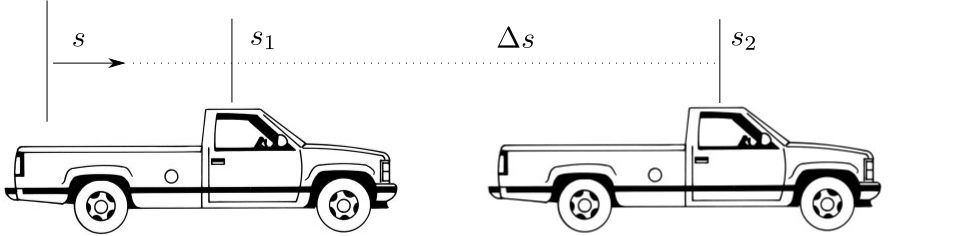
\includegraphics[scale=0.5]{lecture1_fig1.png}\\\\

			\item After 2 hours how far has the truck traveled?\\\\
			
			\item Did you know that you just {\bf integrated}? Why? How?\vspace{40mm}\\
			
			\item This idea is the basis of a family of numerical methods for solving {\bf I}nitial {\bf V}alue {\bf P}roblems known a {\it Forward Integration Techniques}.
		\end{itemize}	
		
		\newpage

\item \textbf{\LARGE Method 1 - Euler's Forward Integration (continued)}\\

	\scalebox{1.5}{$y(x+\Delta x)=y(x) + f(x,y)\Delta x$}\vspace{5mm}\\ 
	\scalebox{1.125}{or with subscript notation shown below}\vspace{5mm}\\ 
	\scalebox{1.5}{$y_{i+1}=y_i + f(x_i,y_i)\Delta x$}\vspace{10mm}\\\\\\
	
	
		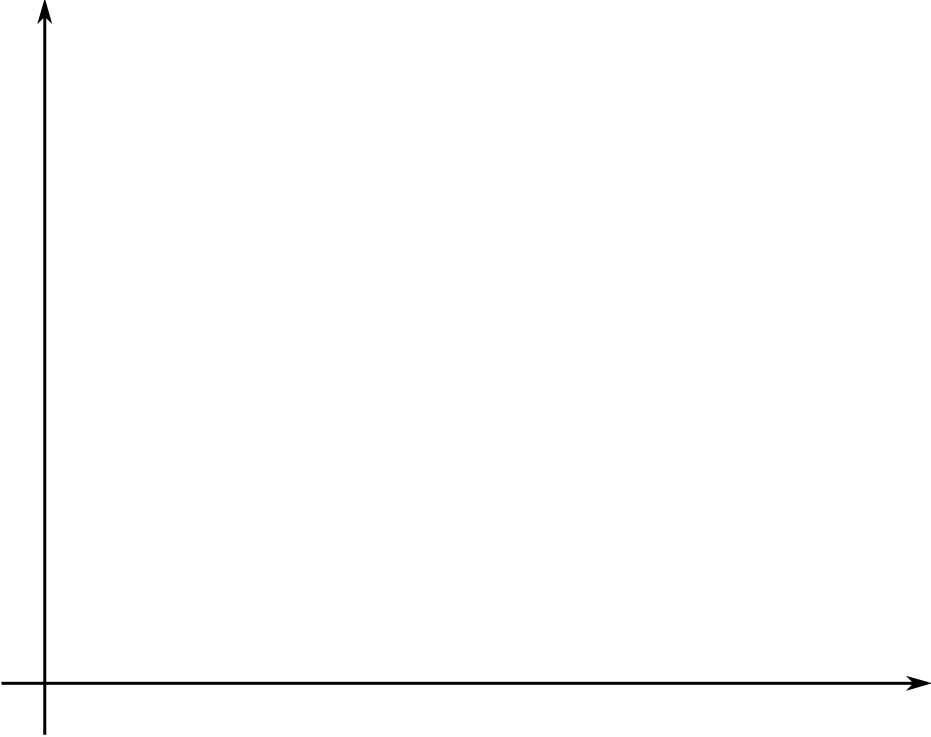
\includegraphics[scale=0.5]{lecture1_fig2.png}\\\\

	
\end{itemize}


	

\end{document}



